
Os comentários dos usuários nas lojas de aplicativos são uma importante fonte de informações para os desenvolvedores, apresentando um vasto conjunto de possíveis requisitos a serem abordados nas versões posteriores dos \textit{apps} \cite{Ciurumelea2017analyzing,Li2018MobileAE,Ortega2015thesis,Palomba2015userreviews,Palompa2018crowdsourcing,Pelloni2018becloma}. Além disso, mesmo aplicações de grandes corporações possuem falhas de acessibilidade \cite{Eler2018mate}. Considerando o cenário apresentado, esta proposta de pesquisa visa investigar o relacionamento dos comentários dos usuários, \textit{commits} e \textit{issues} dos desenvolvedores envolvendo o tema acessibilidade, bem como o quão relevante é este ponto de vista frente ao volume total. O objetivo principal desta pesquisa é a apresentação de um panorama geral sobre esta perspectiva.

A pesquisa visa estender o estudo piloto \cite{ihc2019} que identificou baixo índice de comentários envolvendo este tema, em torno de 1,2\%, em conjunto específico de 701 \textit{apps}. Nessa ocasião foram analisados de forma manual aproximadamente 5000 comentários, considerando apenas as aplicações que possuem código fonte aberto no Github \footnote{https://github.com/} e com versões anteriores de instalação disponíveis no repositório F-Droid\footnote{https://f-droid.org/}.


\section{Estudo Bibliográfico}
O início da pesquisa se dá através de um estudo bibliográfico envolvendo os guias de padrões para acessibilidade internacionais da BBC \cite{bbc} e W3C \cite{wcag}, e suas influências no padrão brasileiro eMAG \cite{emag}. Esta etapa provê o embasamento crítico para avaliar os comentários dos usuários, bem como os \textit{commits} e \textit{issues} dos desenvolvedores.

Além disso, foram analisados artigos envolvendo comentários. Estes estudos apresentam diferentes formas de abordar o tema, considerado como um rico conjunto de informações aos desenvolvedores. Com o advento das lojas de aplicativos, a facilidade em disponibilizar novas versões do software tornou o planejamento das entregas um importante pilar no processo de engenharia de software, apoiado no modelo Ágil de Entregas \cite{manifestoagil}. São encontrados na literatura tanto estudos envolvendo a utilização de comentários de usuários como fonte de requisitos para versões futuras de \textit{apps} \cite{Ciurumelea2017analyzing,Li2018MobileAE,Ortega2015thesis,Palomba2015userreviews}, quanto avaliações de diferentes formas para classificá-los\cite{Panichella2015how,Pelloni2018becloma,Sorbo2017surf}, porém nenhum estudo relacionou estes três itens (comentários, \textit{commits} e \textit{issues}).


\section{Metodologia}
O alvo desta pesquisa são aplicativos Android pelo motivo desta plataforma ter a maior fatia de mercado mundial \cite{ihc2019} e que possuem o código fonte aberto no \textit{Github}, o que permitirá obter as informações disponibilizadas pelos desenvolvedores referentes aos \textit{commits} e \textit{issues}. A lista inicial de \textit{apps} utilizada será a mesma obtida no estudo piloto \cite{ihc2019}, que considerou se a aplicação está disponível no repositório F-Droid. Este requisito visa permitir a evolução desta pesquisa, validando casos de testes envolvendo acessibilidade em diferentes versões dos \textit{apps}.

Será adotada a seguinte metodologia para se alcançar os objetivos deste projeto de pesquisa:

\begin{itemize}
	\item [1] Revisão Bibliográfica: inicialmente será realizada uma etapa de estudos envolvendo os diferentes padrões de acessibilidade da BBC \cite{bbc}, W3C \cite{wcag} e do eMAG \cite{emag}. Esta preparação inicial, já finalizada no momento da Qualificação, visa fornecer embasamentos teóricos que permitirão analisar os resultados obtidos em etapa posterior.
	\item [2] Seleção dos \textit{apps}: será selecionado um conjunto de aplicativos com comentários na loja de (\textit{apps}) \textit{Google Play Store} e com códigos fontes disponíveis no Github. Esta seleção visa verificar posteriormente se o apoio de grandes investidores influencia a acessibilidade do software, bem como é desejo desta pesquisa identificar o panorama para os pequenos desenvolvedores.
	\item [3] Obtenção dos comentários: esta etapa consiste em levantar exemplos de forma automatizada, através de um \textit{crawler} elaborado em linguagem Python. A obtenção destes dados já está concluída no momento da Qualificação, com um total de 214053 comentários, e destes apenas 2663 envolvendo o tema acessibilidade.
	\item [4] Obtenção dos \textit{commits} e \textit{issues}: serão obtidos exemplos dos títulos e detalhes referentes aos \textit{commits} e \textit{issues} cadastrados no \textit{Github} pelos desenvolvedores através de um \textit{crawler} elaborado em linguagem Python. A obtenção destas informações já se encontra concluída no momento da Qualificação, com um total de 767201 commits e 31772 issues.
	Os percentuais dos textos que possuem as palavras-chave do estudo piloto identificados em momento da coleta foram de 842 (2.46\%) e 3149 (9,91\%), respectivamente.
	\item [5] Definição das palavras-chave: nesta etapa serão revisados os conjuntos de palavras-chave inicialmente estabelecidos durante o estudo piloto \cite{ihc2019}, e que consideram o padrão da BBC. Nesta revisão serão considerados os conhecimentos obtidos na etapa de Revisão Bibliográfica, expandindo o conjunto para os demais padrões citados nesta proposta de pesquisa (W3C e eMAG).
	\item [6] Filtragem dos comentários, \textit{commits} e \textit{issues}: em seguida serão filtrados exemplos de acordo com o conjunto de palavras estabelecido na etapa anterior.
	\item [7] Análise dos dados: finalmente serão analisadas as amostras filtradas. Os percentuais obtidos no estudo piloto serão estendidos para os \textit{commits} e \textit{issues} considerando o novo conjunto de palavras-chave. Será verificado se o mesmo comportamento dos comentários (baixo índice e notas inferiores para casos específicos de reclamações) é refletido para os outros dois itens, correlacionando desta forma os três conjuntos de dados.
	Durante a etapa de análise, poderão ser realizadas revisões manuais que validem percentuais fora do padrão esperado, de acordo com o estudo piloto \cite{ihc2019}. De acordo com \cite{Panichella2015how}, os usuários aplicam o mesmo padrão de resposta quando a sua intenção é de reportar um problema.	
\end{itemize}


\section{Cronograma}

Segue abaixo o cronograma esperado para esta proposta de pesquisa:

*********************

cronograma com imagem

*********************


\begin{figure}[!htb]
	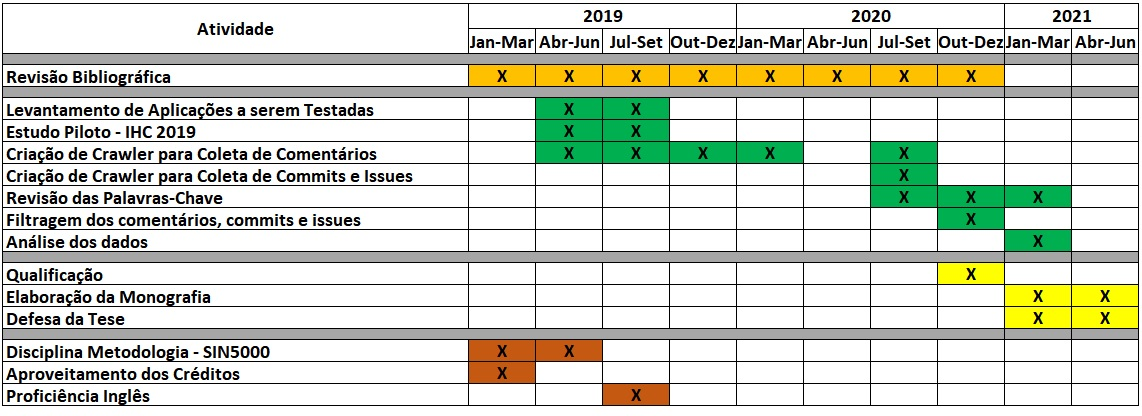
\includegraphics[scale=0.55]{imagens/Cronograma-v1.jpg}
	\caption{Cronograma - Imagem}
	\label{fig:cronograma}
\end{figure}

%%%%%%%%%%%%%%%%%%%%%%%%%%%
%%Tabela 1 - 10 trimestres%
%%%%%%%%%%%%%%%%%%%%%%%%%%%

********

tabela 1

********

\begin{table}[htbp]
	\centering
	\caption{Cronograma - tabela teste apenas - modelo PPGSI}
	\begin{tabular}{p{1in} p{1in} p{1in} p{1in} } \hline
		
		Atividade														& Jan-Mar	& Cabeçalho 3	& Cabeçalho 4 \\ \hline
		Revisão Bibliográfica											& número & número	& número \\ 
		Levantamento de Aplicações a serem Testadas (Acessibilidade)	& número & número	& número \\ 
		Texto	& número & número	& número \\ 
		Texto	& número & número	& número \\ 
		Texto	& número & número	& número \\ \hline
		
	\end{tabular}
	\label{tab:cronogramappgsi}
	\source{Marcelo Fantinato, 2015}
\end{table}


*******************************************

tabela 2 - não contem os trimestres de 2021

*******************************************


\begin{table}[htbp]
	\centering
	\caption{Cronograma 2019 / 2020}
	\label{tab:Cronograma}
	\begin{tabular}{p{3.40in} p{0.20in} p{0.20in} p{0.20in} p{0.20in} p{0.20in} p{0.20in} p{0.20in} p{0.20in}} \hline
		%	\begin{tabular}{lcccccccc}
		\textbf{Atividade}							& Jan Mar & Abr Jun & Jul Set & Out Dez & Jan Mar & Abr Jun & Jul Set & Out Dez \\ \hline
		Revisão Bibliográfica						& X		  & X 	 	& X		  & X  		& X  	  & X  		&         & 	    \\ 
		Levantamento de Aplicações a serem Testadas	& 		  & X	    & X		  &    		&  		  &  	    & 		  & 	    \\ 
		Teste de Falhas nas Aplicações	  			&  		  & 	    & X		  & X		&    	  &  	    &  	      & 		\\ 
		Criação de Crawler - Coleta de Comentários	&  		  & X       & X		  & X		&    	  &  	    &  	      & 		\\ 
		Identificação Parceria - Execução de Testes	&  		  & 	    & X		  & X		&    	  &  	    &  	      & 		\\ 
		Testes Utilizando PLN sobre Dados Coletados &  		  & 	    & X		  & X		& X  	  &  	    &  	      & 		\\
		Inclusão de Comentários para Aplicações		&  		  & 	    &  		  & X		& X  	  & X	    &  	      & 		\\
		Análise das Ações dos Desenvolvedores		&  		  & 	    &  		  &  		&    	  & X	    & X	      & 		\\ \hline
		Qualificação								&  		  & 	    &  		  &  		& X  	  &  	    &  	      & 		\\
		Elaboração da Monografia					&  		  & 	    &  		  &  		& X  	  & X	    & X	      & 		\\
		Defesa da Tese								&  		  & 	    &  		  &  		&    	  &  	    & X	      & X   	\\ \hline
		%Disciplina Metodologia - SIN5000			& X		  & X       &  		  &  		&    	  &  	    &  	      & 		\\
		Proficiência Inglês							&  		  & 	    & X		  & X		&    	  &  	    &  	      & 		\\
	\end{tabular}
\end{table}


*******************

tabela 3 - 30 meses

*******************



%%%%%%%%%%%%%%%%%%%%%%
%%Tabela 2 - 30 meses%
%%%%%%%%%%%%%%%%%%%%%%

\begin{table*}[!htb]
	\centering
	\caption{Cronograma - tabela teste apenas - versão 2}
	\label{tab:cronograma}
	\resizebox{\textwidth}{!}{ % abre resizebox, setar tabela da largura da página.
		\begin{tabular}{lcccccccccccccccccccccccccccccccc}
		\hline
		Atividade             							& 1 & 2 & 3 & 4 & 5 & 6 & 7 & 8 & 9 & 10 & 11 & 12 & 11 & 12 & 13 & 14 & 15 & 16 & 17 & 18 & 19 & 20 & 21 & 22 & 23 & 24 & 25 & 26 & 27 & 28 & 29 & 30 \\
		\hline
		Levantamento
		                      							&   &   &   &   &   &   &   &   &   &    &    &    &    &    &    &    &    &    &    &    &    &    &    &    &    &    &    &    &    &    &    &    \\
		Crawler Comentários
		                      							&   &   &   &   &   &   &   &   &   &    &    &    &    &    &    &    &    &    &    &    &    &    &    &    &    &    &    &    &    &    &    &    \\
		Estudo Piloto
		                      							&   &   &   &   &   &   &   &   &   &    &    &    &    &    &    &    &    &    &    &    &    &    &    &    &    &    &    &    &    &    &    &    \\
		Crawler Commits
														&   &   &   &   &   &   &   &   &   &    &    &    &    &    &    &    &    &    &    &    &    &    &    &    &    &    &    &    &    &    &    &    \\
		Crawler Issues
														&   &   &   &   &   &   &   &   &   &    &    &    &    &    &    &    &    &    &    &    &    &    &    &    &    &    &    &    &    &    &    &    \\
		\end{tabular}
	}
\end{table*}


\section{Contribuições}
As principais contribuições esperadas desta pesquisa são as evidências de que não só as aplicações móveis são pouco acessíveis, mas que também os requisitos relacionados à acessibilidade digital raramente são abordados durante a evolução de uma aplicação móvel.
Os resultados desta pesquisa podem contribuir com os estudos relacionados à acessibilidade digital em aplicações móveis e fomentar pesquisas e ações voltadas à conscientização e treinamento de desenvolvedores, e igualmente a criação de novos recursos para
a implementação e avaliação de acessibilidade digital.
Como contribuições adicionais entregues, podemos citar:

\begin{itemize}
	\item Conjunto de dados de comentários, \textit{commits} e \textit{issues} para posteriores estudos relacionados;
	\item Evolução dos conjuntos de palavras-chave relacionadas à acessibilidade, expandindo o mesmo para os padrões W3C e eMAG;
	\item Código fonte em Python que permita realizar a obtenção de comentários do \textit{Google Play Store}, dos \textit{commits} e \textit{issues} cadastrados no Github.
\end{itemize}



%3.1
%Descrição mais detalhada do que iremos fazer
%1 - pequisa introdução retomando o assunto: visto que os comentários são interessantes para os desenvolvedores, tem muitas informações para eles melhorarem, os motivam e que as aplicações têm pouca acessibilidade, queremos verificar se as pessoas enviam os comentário
%2 - queremos investigar se as pessoas comentam sobre acessibilidade dos repositórios
%3 - vamos detalhar nosso estudo para chegar a esta conclusão
%4 - estudo bibliográfico:
%estudar os guias de acessibilidade
%selecionar os aplicativos que serão analisados
%introdução
%metodologia
%selecionar os apps
%coletar os comentários
%filtrar os comentários
%keywords
%análise manual
%analisar comentários
%usar estatísticas: porquê? o que queremos com elas?
%porcentagem de comentários que envolvem acessibilidade
%porcentagens: basicamente aquilo que já está no artigo referente
%inserir gráficos, como no artigo
%PLN: por que utilizar PLN? Precisamos pensar o motivo
%Usos para PLN: dividir em tópicos, análise de sentimentos, neste sentido, podemos citar o artigo do Panichella
%Seria interessante fazermos uma análise temporal? Comentários ao longo do tempo. Analisar 3 meses seguidos? Comparar com as quantidades de comentários levantados no passado.
%olhar os dados e pensar
%Como estamos fazendo um estudo exploratório, não teríamos hipóteses a serem citadas
%O que queremos com todo este estudo: mostrar um panorama geral sobre isso tudo e tirar uma conclusão se isso é bastante, se é pouco


%3.2
%Citar as atividades já realizadas
%Descrever que já fizemos um estudo piloto motivacional: IHC2019
%descrever sucintamente, fazendo uma referência para o artigo

%3.3
%Cronograma
%listar as atividades, que estão relacionadas com tudo, incluindo o estudo piloto, colocando por mês ou bimestre, desde quando entrei como regular
%parecido com o que foi apresentado no ppt, quebrando um pouco mais do que por trimestre
%fizemos tudo isso, mas o quê queremos mais? analisamos poucos aplicativos, apenas 700, podemos ampliar este número de apps. Depois do estudo piloto aprendemos como fazer, agora queremos repetir para um número maior de aplicativos
%temos 2 opções: falar que vamos fazer novas análises, não feitas ainda no artigo, ou então vamos aprofundar mais as análises já feitas no artigo
%conclusão: tudo isso já fiz, mas falta esta parte ainda
%opção 1: melhorar o artigo fazendo estas análises, e daí termina o mestrado
%opção 2: ter uma outra estratégia, como por exemplo pegar os top 20 de cada categoria, pegar os tops pode me dar um resultado enviezado, já que os tops têm altos valores aportados (recursos) e por isso podem ter um retorno bom dos comentários. Precisamos saber o caso normal dos desenvolvedores
%fazer análises comparativas dos tops, aliatoriamente com alguns do meio, outros menos baixados, podemos identificar diferenças por serem tops, ou até mesmo não encontrar diferenças

%entrar na estratégia: quais serão as seleções que serão feitas, no estudo piloto tem descrito a estratégia que foi utilizada no artigo: pegou o que estava no github, aqueles que estavam no F-Droid, e então obteve os comentários. Até a qualificação foram feitos todos os itens, depois da qualificação temos novamente os passos, agora seguindo a estratégia que pretendemos utilizar

%importante: no estudo piloto tivemos uma análise manual sobre 5000 comentários. Podemos extrapolar as interpretações sobre as palavras chaves em todos os comentários que identificarmos, já que os volumes possivelmente serão maiores. mas devemos perder muito com esta extrapolação.
%outra opção seria a utilização de PLN para saber, mas precisaríamos validar com a Sarajane ou com o Ivandré. O estudo piloto também pode direcionar a exclusão de falsos positivos (ex: palavra (header). O estudo piloto serviu para identificarmos falsos positivos, principais keywords, montar uma estatística

%e no fim as considerações finais, retomar o que foi já feito. Muito do que está no artigo serve e me guiará no que deve ser feito.
